% **************************************************
%   Wichtig für die verwendung der hsrmreport-Klasse!
%   
%   Die Datei hsrmreport.cls muss in dem selben Ordner sein
%   wie die .tex Datei die diese Klasse verwenden möchte.
%
%   Desweiteren ist die Dokumentenklasse nach aktuellem 
%   noch ohnen Optionen, sprich Zweiseitig, änderung 
%   der Schriftgröße oder ähnliches. Ich werde versuchen 
%   diese Features hinzu zufügen sobald es mir möglich ist. 
%
%   Falls Ihr Probleme, Anregungen oder Verbesserungen habt,
%   könnt ihr mir das gerne mitteilenen.
%
%   Es kann sein das ihr evtl. manche Packete noch installieren 
%   müsst bevor die Klasse Fehlerfrei funktioniert.
%   Meldungen wie "Command terminated with space." können ignoriert werden.
%
%   Ich werde auch eine Übersicht aller Pakete schreiben, die ich verwendet habe.
%      
%
%   E-Mail: timjonas.wechler@student.hs-rm.de
% **************************************************


\documentclass{hsrmreport}
% **************************************************
% Ihr könnte die Angaben der TITELSEITE hier ändern
% **************************************************
\newcommand{\titel}{Versuch 1}
\newcommand{\studiengang}{Angewandte Pyhsik}
\newcommand{\studienrichtung}{}
\newcommand{\dokumentenart}{Praktikumsbericht}
\newcommand{\kurs}{LV:\ Elektronik 1 Praktikum}
\newcommand{\versuchsdurchfuehrung}{30. November 2020}

%Falls ihr weniger als vier Studenten seit könnt ihr dies Einträge die zu viel sind einfach löschen. 
%Ein Feature für das angeben der Mat.Nr. ist noch in Arbeit. 
\newcommand{\studentA}{Cassel, Niclas}
\newcommand{\matStudentA}{(1110348)}
\newcommand{\studentB}{Wechler, Tim-Jonas}
\newcommand{\matStudentB}{(1137877)}
\newcommand{\studentC}{}
\newcommand{\matStudentC}{}
\newcommand{\studentD}{}
\newcommand{\matStudentD}{}


% Mit dem Befehl \today wird immer das aktuelle Datum auf der Titelseite ausgebeben.
% Wenn dies nicht erwünscht ist einfach manuell das gewünschte Datum eintragen.
\newcommand{\datum}{\today}



\begin{document}
    % **************************************************
    %
    %   ALLES zwischen hier und dem Begin des Berichts 
    %   nicht ändern, außer ihr wisst was ihr tut ;). 
    %
    % **************************************************

    % Title 
    \frontpage

    %Römischen Seitenzahl
    \pagenumbering{Roman}
    
    %Inhaltsverzeichnis
    \tableofcontents

    %Abbildungsverzeichnis
    %\listoffigures

    %Tabellenverzeichnis
    %\listoftables

    
    \clearpage

    %Normale Seitenzahlen
    \pagenumbering{arabic}

    %Das seitenLayout mit Kapitel und Unterkapitel im Header jeder Seite des Berichts
    \pagestyle{scrheadings}

    % **************************************************
    %
    % HIER BEGINNT DER BERICHT
    %
    % **************************************************

    
        \chapter{Vorbereitung}
    Für eine zielorientierte Durchführung des Versuchs 1 in Elektronik 1 Praktikum haben wir das Ziel definiert.
    \section{Ziele des Versuchs}
        Das Ziel des Versuchs ist, der grundsätzliche Umgang mit LTspice zu lernen. Damit ist gemeint dass, mit Beendigung des Versuchs erlangte Wissen aus der Simulation auf praktische Schaltungen angewendet werden kann. 
    \section{Begriffserklärung}
        Im Folgenden werden einige Begriffe näher erklärt die essentiel für diesen Versuch sind.
        Als erstes werden die Begriffe Gleich- und Wechselspannung erklärt und auf die Unterschiede hingewiesen. 
        Im Anschluss werden dann die Begriffe Effektivwert und Spitzenwert erklärt. Zum Schluss wird dann noch auf Spannungsteiler und Potentiometer eingegangen.  
        \subsection{Gleichspannung und Wechselspannung}
        Um die Begriffe Gleichspannung und Wechselspannung zu erklären nehmen zunächst einen Schaltkreis \frefadd{fig:stromkreis}{links}. Redet man von \textbf{Gleichspannung}, so liefert die Spannungsquelle(\(U_1\)) eine konstante Spannung \figrefadd{fig:spannung}{links} durch ein Potentialunterschied an dem Ein- und Ausgang der Spannungsquelle.
        Bei der \textbf{Wechselspannung}, wie der Name schon sagt, wechselt die Spannung. Das Schaltbild unterscheidet sich im wesentlichen nur von der Spannungsquelle \figrefadd{fig:stromkreis}{rechts}. Das abwechsel der Spannung ist im Normalfall mit einer festen Frequenz in einem sinuförmigen Verlauf \frefadd{fig:spannung}{rechts}. 

        \begin{figure}[ht]
            \centering
            \begin{circuitikz}[european resistors,european voltage source]
                \draw (0,0) to[vsource,V=$U_1$] (0,3) -- (2,3)
                    to[R,R=$R_1$](2,0) -- (0,0);
            \end{circuitikz}
            \hspace{1cm}
            \begin{circuitikz}[european resistors,european voltage source]
                \draw (0,0) to[vsource,sV=$U_2$] (0,3) -- (2,3)
                    to[R,R=$R_2$](2,0) -- (0,0);
            \end{circuitikz}
            \caption{Stromkreis mit einer Spannungsquelle($U$) und einem Verbraucher($R$)\\links: Gleichspannung, rechts: Wechselspannung}
            \label{fig:stromkreis}
        \end{figure}

        \begin{figure}[ht!]
            \centering
            
            \begin{minipage}[t]{.45\linewidth}
                \centering
                \begin{tikzpicture}

                    % horizontal axis
                    \draw[->] (0,0) -- (6.25,0) node[anchor=north] {$t/s$};
                    % labels
                    \draw	(0,0) node[anchor=east] {0}
                            (1,0) node[anchor=north] {1}
                            (2,0) node[anchor=north] {2}
                            (3,0) node[anchor=north] {3}
                            (4,0) node[anchor=north] {4}
                            (0,2) node[anchor=east] {5};
                    %grid
                    \draw[step=1cm,gray,dotted] (0.1,-2.9) grid (5.9,3.9);            
        
                    % vertical axis
                    \draw[->] (0,-3) -- (0,4) node[anchor=east] {$U/V$};
                                
                    % Us
                    \draw[thick] (0,2) -- (6,2);
                    \draw (2.5,2.5) node {$U_1$}; %label
                            
                \end{tikzpicture}
                
            \end{minipage}
            \begin{minipage}[b]{.45\linewidth}
                \centering
                \begin{tikzpicture}

                    % horizontal axis
                    \draw[->] (0,0) -- (6.25,0) node[anchor=north] {$t/s$};
                    % labels
                    \draw	(0,0) node[anchor=east] {0}
                            (1,0) node[anchor=north] {1}
                            (2,0) node[anchor=north] {2}
                            (3,0) node[anchor=north] {3}
                            (4,0) node[anchor=north] {4}
                            (0,2) node[anchor=east] {5}
                            (0,-2) node[anchor=east] {-5};
                    %grid
                    \draw[step=1cm,gray,dotted] (0.1,-2.9) grid (5.9,3.9);            
        
                    % vertical axis
                    \draw[->] (0,-3) -- (0,4) node[anchor=east] {$U/V$};
                                
                    % Us
                    \draw[thick] (0,0) sin (1,2) cos (2,0) sin (3,-2) cos (4,0) sin (5,2) cos (6,0);
                    \draw (1,2.5) node {$U_2$}; %label
                            
                \end{tikzpicture}
            \end{minipage}
            
            \caption{links: Spanungsverlauf bei Gleichspannung, rechts: Spannungsverlauf bei Wechselspannung}
            \label{fig:spannung}
        \end{figure}
       

        \subsection{Effektivwert und Spitzenwert}
            Der \textbf{Effektivwert} beschreibt den quadratischen Mittelwert physiklischer Größen, die sich über die Zeit verändern. Hat man ein Schaltkreis mit Wechselspannung \figrefadd{fig:stromkreis}{rechts}, so beschreibt der Effektivwert die gleiche Leistung, die über den Verbraucher abfällt, wie bei einem Schaltkreis mit Gleichspannung \figrefadd{fig:stromkreis}{links}.
            Der \textbf{Spitzenwert} ist der Wert für die Amplitudenauslenkung, von einem Hochpunkt bis zu einem Tiefpunkt. Auch dieser Wert taucht nur bei verwendung von Wechselspannung auf. Als Beispiel in einer Wechselspannung mit 5 V \figrefadd{fig:spannung}{rechts} liegt der Wert bei $10\ V$.

        \subsection{Spannungsteiler und Potentiometer}
            \textbf{Spannungsteiler} gibt es in zwei Varianten. Zum einen den unbelasteten Spannungsteiler und den belasteten Spannungsteiler. Der unbelastete Spannungsteiler besteht aus zwei in Reihe geschalteten Widerstände. Die Verteilung von Strom und Spannung im unbelasteten Spannungsteiler ist mit der Reihenschaltung gleich zu setzten. 
            Der belastete Spannungsteiler hat den Unterschied, dass bei einem der beiden vorherigen Widerstände ein weiterer parallel geschalten wird. Dieser  dirtte Widerstand nennt man auch Lastwiderstand.
            Durch diesen weiteren Widerstand wird die Schaltung zu einer gemischten Schaltung aus Parallel- und Reihenschaltung. Durch eine vergrößerung der Last an dem Lastwiderstand tretten nun gewisse Veränderungen auf, die im Folgenden kurz genannt werden. 
            \begin{enumerate}
                \item Der Gesamtwiderstand der Schaltung wird kleiner.
                \item Der Gesamtstrom der Schaltung steigt an.
                \item Die Teilspannung an dem parallel geschalteten Widerstand wird kleiner.
                \item Die Teilspannung an dem in Reihe geschalteten Widerstand wird größer.
            \end{enumerate} 
            %\hyperref{https://www.elektronik-kompendium.de/sites/slt/0201111.htm}

            Ein \textbf{Potentiometer} ist ein verstellbarer Spannungsteiler. Hier wird durch drehen oder verschieben der Lastwiderstand verändert. 

    \section{Berechnung des Effektivwerts}
        Als nächste wird der Effetivwert berechnet mit dem allgemeinen Ansatz, gefolgt von dem Effektivwert Bei einer symmetrischen rechteckförmigen Wechselspannung und einer symmetrischen dreieckförmigen Wechselspannung. Zum Schluss wird die Gleichung für den Spannungsteiler aufgestellt.
        \subsection{Allgemeiner Ansatz}
            Die allgemeine Formel für die Berechnung des Effektivwerts sieht wie folgt aus.
            \begin{equation}
                U_{eff}=\sqrt{\frac{1}{T}\cdot\int_{t_0}^{t_0+T} u^2(t)\partial t}
            \end{equation}

            Setzt man nun für $ u(t) = û\cdot sin(\omega t)$ ein, erhält man folgendes.
            \begin{equation}
                U_{eff}=\sqrt{\frac{1}{T}\cdot\int_{t_0}^{t_0+T} û^2\cdot sin^2(\omega t)\partial t}
            \end{equation}
Jetzt kann man das Integral auflösen.
\begin{equation}
    U_{eff}=\sqrt{\frac{û^2}{T}\cdot\left[\frac{t}{2} - \frac{\sin(2\omega t)}{4\omega}\right]_{t_0}^{t_o+T}}
    \label{ansatz}
\end{equation}
Im Anschluss werden die Grenzen noch eingesetzt und vereinfacht. 
\begin{gather}
    t_0 = 0\, s\\
    \omega = 2\pi\frac{1}{T}\\
    U_{eff}=\sqrt{\frac{û^2}{T}\cdot\left(\frac{T}{2}-\frac{sin\left(\frac{4\pi}{T} T\right)}{\frac{8\pi}{T}}\right)}
\end{gather}
Da $sin(0) = sin(2\pi) = sin(4\pi) = 0$ entspricht. 
\begin{gather}
    U_{eff}=\sqrt{\frac{û^2}{T}\cdot\frac{T}{2}}\\
    U_{eff}=\frac{û}{\sqrt{2}}\\
    U_{eff}=\frac{1\, V}{\sqrt{2}} = 0,707\, V
\end{gather}
        \subsection{Recheckförmige Wechselspannung}
            Unter Annahme für die rechteckigförmige Wechselspannung mit der Gleichung
            \begin{equation}\label{equ:rechteck}
                U_{eff}=\sqrt{\frac{1}{T}\cdot\left(\int_{t_0}^{t_0+\frac{T}{2}} u^2(t)\partial t + \int_{t_0+\frac{T}{2}}^{t_0+T} u^2(t)\partial t\right)}
            \end{equation} 
            und dass 
            \begin{align}
                u(t)=û  &\hspace{1cm}0 \leq t \leq \frac{T}{2}\\
                u(t)=0 &\hspace{1cm} \frac{T}{2} \leq t \leq T
            \end{align}    
            erhält man allgemeingültig 
            \begin{gather}
                U_{eff}=\sqrt{\frac{1}{T}\cdot\left(\int_{0}^{\frac{T}{2}} u^2(t)\partial t + \int_{\frac{T}{2}}^{T} u^2(t)\partial t\right)}    \\
                U_{eff}=\sqrt{\frac{û^2}{T}\cdot\left(\int_{0}^{\frac{T}{2}} \partial t + \int_{\frac{T}{2}}^{T}\partial t\right)}    \\
                U_{eff}=\sqrt{\frac{û^2}{T}\cdot\left(\big[t\big]_{0}^{\frac{T}{2}} + \big[t\big]_{\frac{T}{2}}^{T}\right)} \\  
                U_{eff}=\sqrt{\frac{û^2}{T}\cdot\left(\frac{T}{2}+T-\frac{T}{2}\right)} \\
                U_{eff}=û\sqrt{1} = û = 1V
            \end{gather}
        \subsection{dreieckförmige Wechselspannung}   
       
            In diesem Fall gilt:
            \begin{align}
                u(t)=û\left(1-\frac{2t}{T}\right)  &\hspace{1cm}0 \leq t \leq \frac{T}{2}\\
                u(t)=û\left(\frac{2(t-\frac{T}{2})}{T}\right) &\hspace{1cm} \frac{T}{2} \leq t \leq T
            \end{align}
            Für diese Betrachtung kann man die Gleichung ~\ref{equ:rechteck} benutzen. Setzt man die Bedingung ein erhält man folgendes.
            \begin{gather}
                U_{eff}=\sqrt{\frac{û^2}{T}\cdot\left(\int_{0}^{\frac{T}{2}} \left(1-\frac{2t}{T}\right)^2\partial t + \int_{\frac{T}{2}}^{T} \left(\frac{2(t-\frac{T}{2})}{T}\right)^2\partial t\right)}    \\
                U_{eff}=\sqrt{\frac{û^2}{T}\cdot\left(\left[\frac{4t^3}{3T^2}-\frac{2t^2}{T}+t\right]_{0}^{\frac{T}{2}} + \left[\frac{4t^3}{3T^2}-\frac{2t^2}{T}+t\right]_{\frac{T}{2}}^{T}\right)}\\
                U_{eff}=\sqrt{\frac{û^2}{T}\cdot\left(\frac{4T^3}{3T^2}-\frac{2T^2}{T}+T \right)}\\
                U_{eff}=\sqrt{\frac{û^2}{T}\cdot\left(\frac{4}{3}T-{2T}+T \right)}\\
                U_{eff}=\sqrt{\frac{û^2}{3}}\\
                U_{eff}=\frac{û}{\sqrt{3}}\\
                => U_{eff}=\frac{1\,V}{\sqrt{3}}= 0,578\,V
            \end{gather}
        \subsection{Spannungsteiler}
            Die Formel für den Spannungsteiler ist folgende.
            \begin{equation}
                \frac{U_2}{U}= \frac{R_2}{R_1+R_2}
            \end{equation}

        


            
        \chapter{Aufgaben}
Bei den Aufgaben werden mit LTSpice Schaltungen zusammengestellt, welche dann praktisch im Labor nachgebaut werden können. In den folgenden Aufgaben werden verschiedene Schaltungen wie Signalquellen, Spannungsteiler und Potentiometer zusammengestellt. 

\section{Signalquellen}
Hier ist der Aufbau einer einfachen Signalquelle zu sehen, welche eine Spannung von 1V besitzt.
\begin{figure}[h!]
\centering
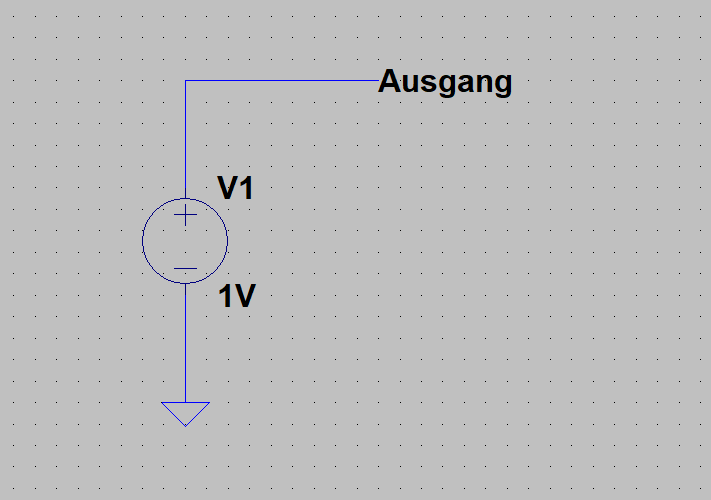
\includegraphics[scale=1]{21.PNG}
\caption{Darstellung einer Signalquelle in LTSpice}
\label{fig: Signalquelle}
\end{figure}
\newpage
Im Folgenden werden mit der Schaltung \fref{fig: Signalquelle}, verschieden Kurvenformen dargestellt und mit den jeweiligen Werten in LTSpice simuliert:



\subsection{Gleichspannungsquelle}
Folgender LTSpice Simulation und Graph wird durch eine Gleichspannungsquelle erzeugt.
\begin{figure}[ht!]
\centering
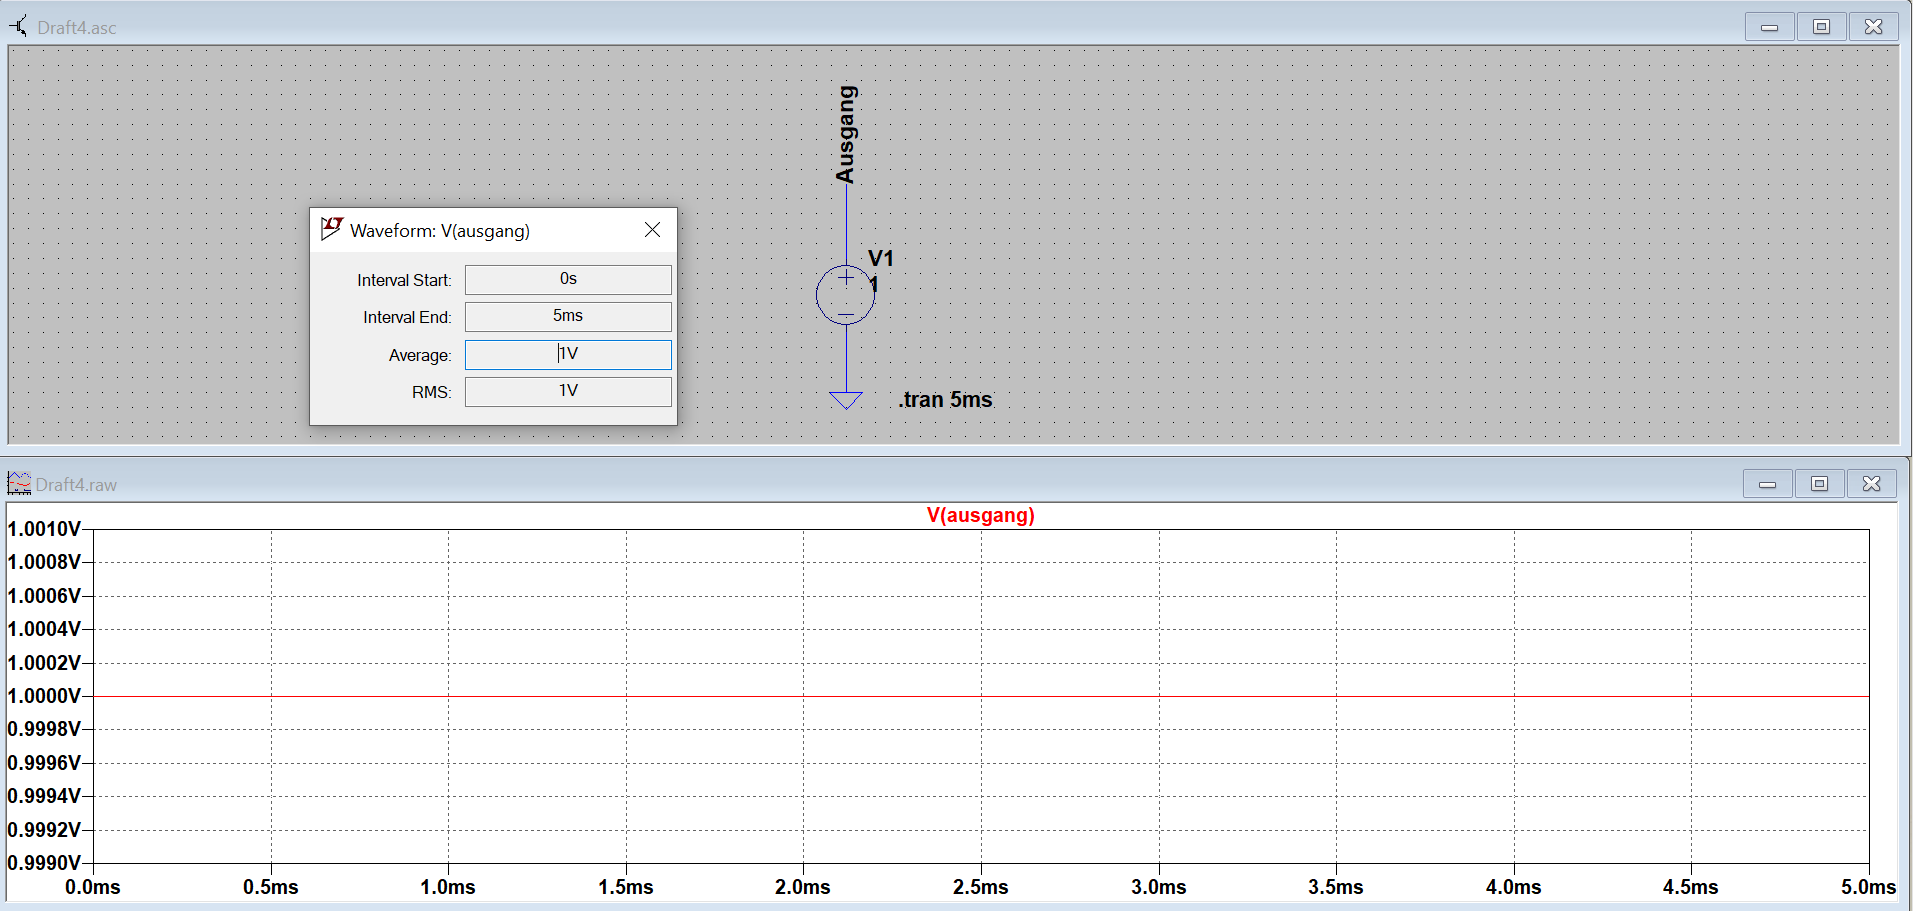
\includegraphics[scale=0.5]{211.PNG}
\caption{Gleichspannungsquelle $U=1V$}
\end{figure}

\subsection{Signussignal}
Um bei der folgenden Simulation ein richtiges Signal heraus zu bekommen, muss die $Periode(T)=1ms$ in die Frequenz f umgerechnet werden.
\begin{equation}
f=\frac{1}{T}=\frac{1}{10^{-3}}=1000Hz
\end{equation}
Folgender LTSpice Simulation und Graph wird durch die Werte erzeugt.
\begin{figure}[h!]
\centering
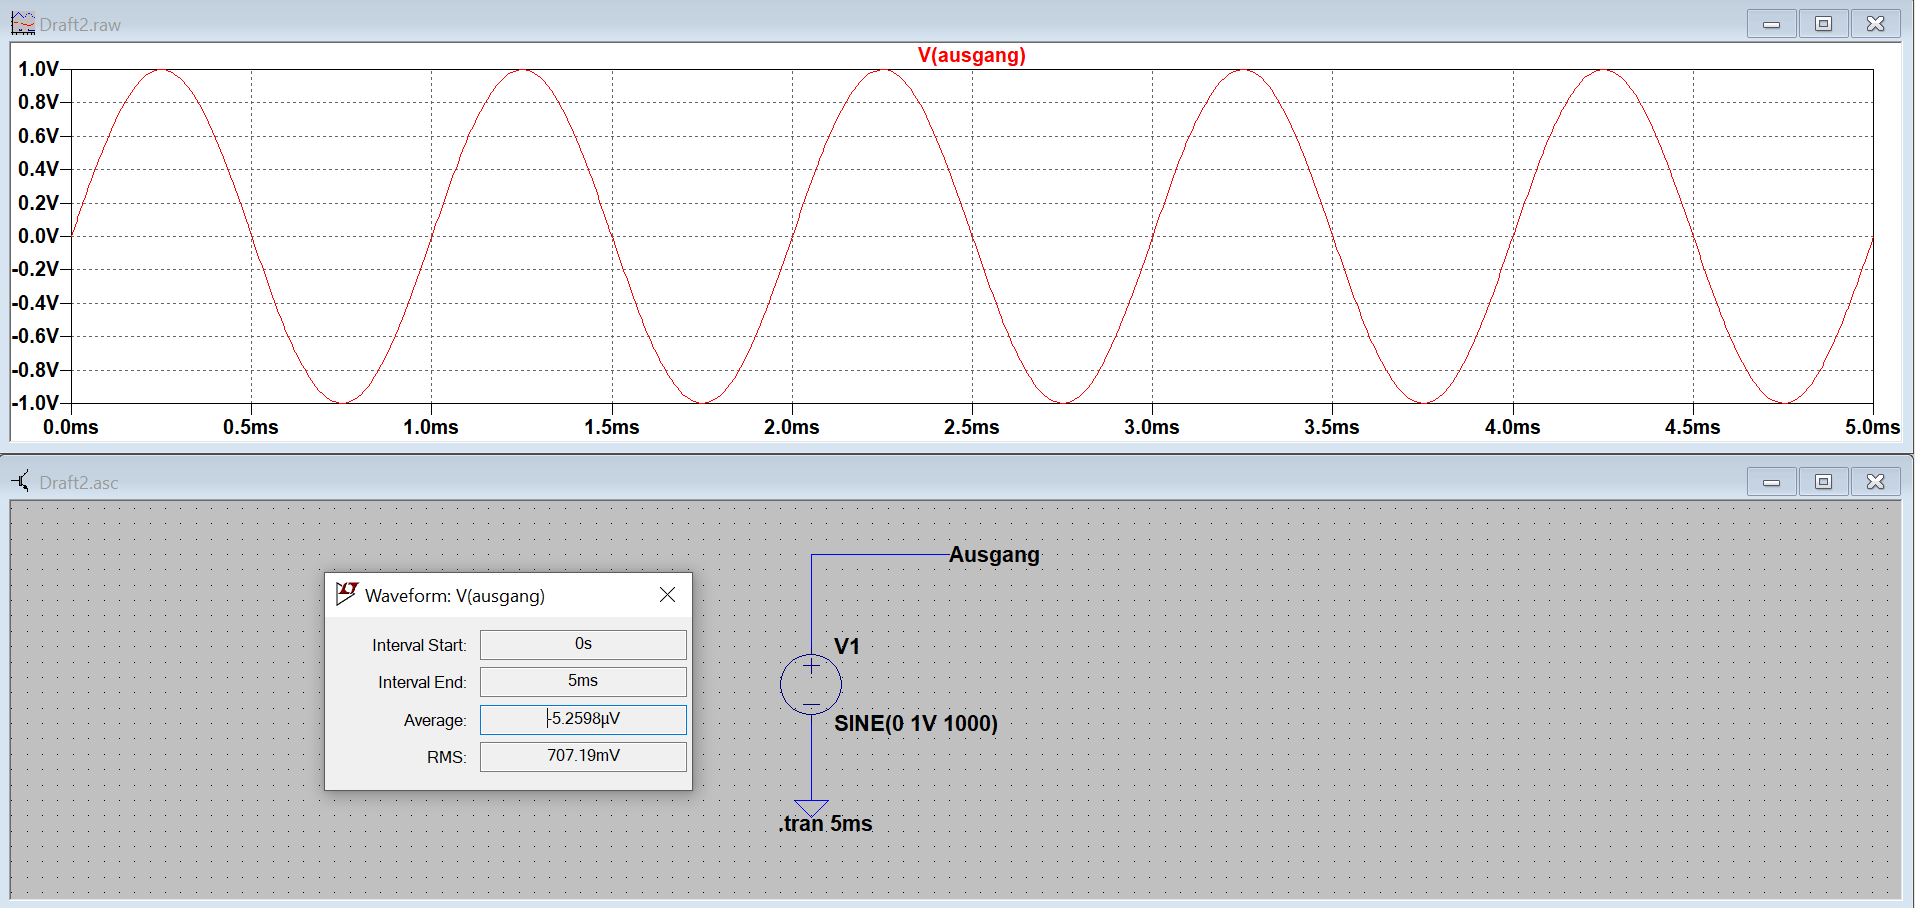
\includegraphics[scale=0.5]{212.PNG}
\caption{Sinussignal mit $\^{U}=1V$ und $T=1ms$}
\label{fig: Sinussignal}
\end{figure}
\newpage

\subsection{Symmetrisches Rechtecksignal}
Zum Darstellen eines symmetrischen Recktecksignals wird der $T_{rise}$ und $T_{fall}$ Wert angepasst. Dieser liegt in der Simulation bei jeweils 1ns. Die Spannungsquelle wird in den Pulse-Mode gestellt und die Werte für $\^{U}$,$T_{on}$ und f eingetragen \fref{fig: symRechtecksignal}. Dabei ergibt sich folgende LTSpice Simulation und Graph. 
\begin{figure}[ht!]
\centering
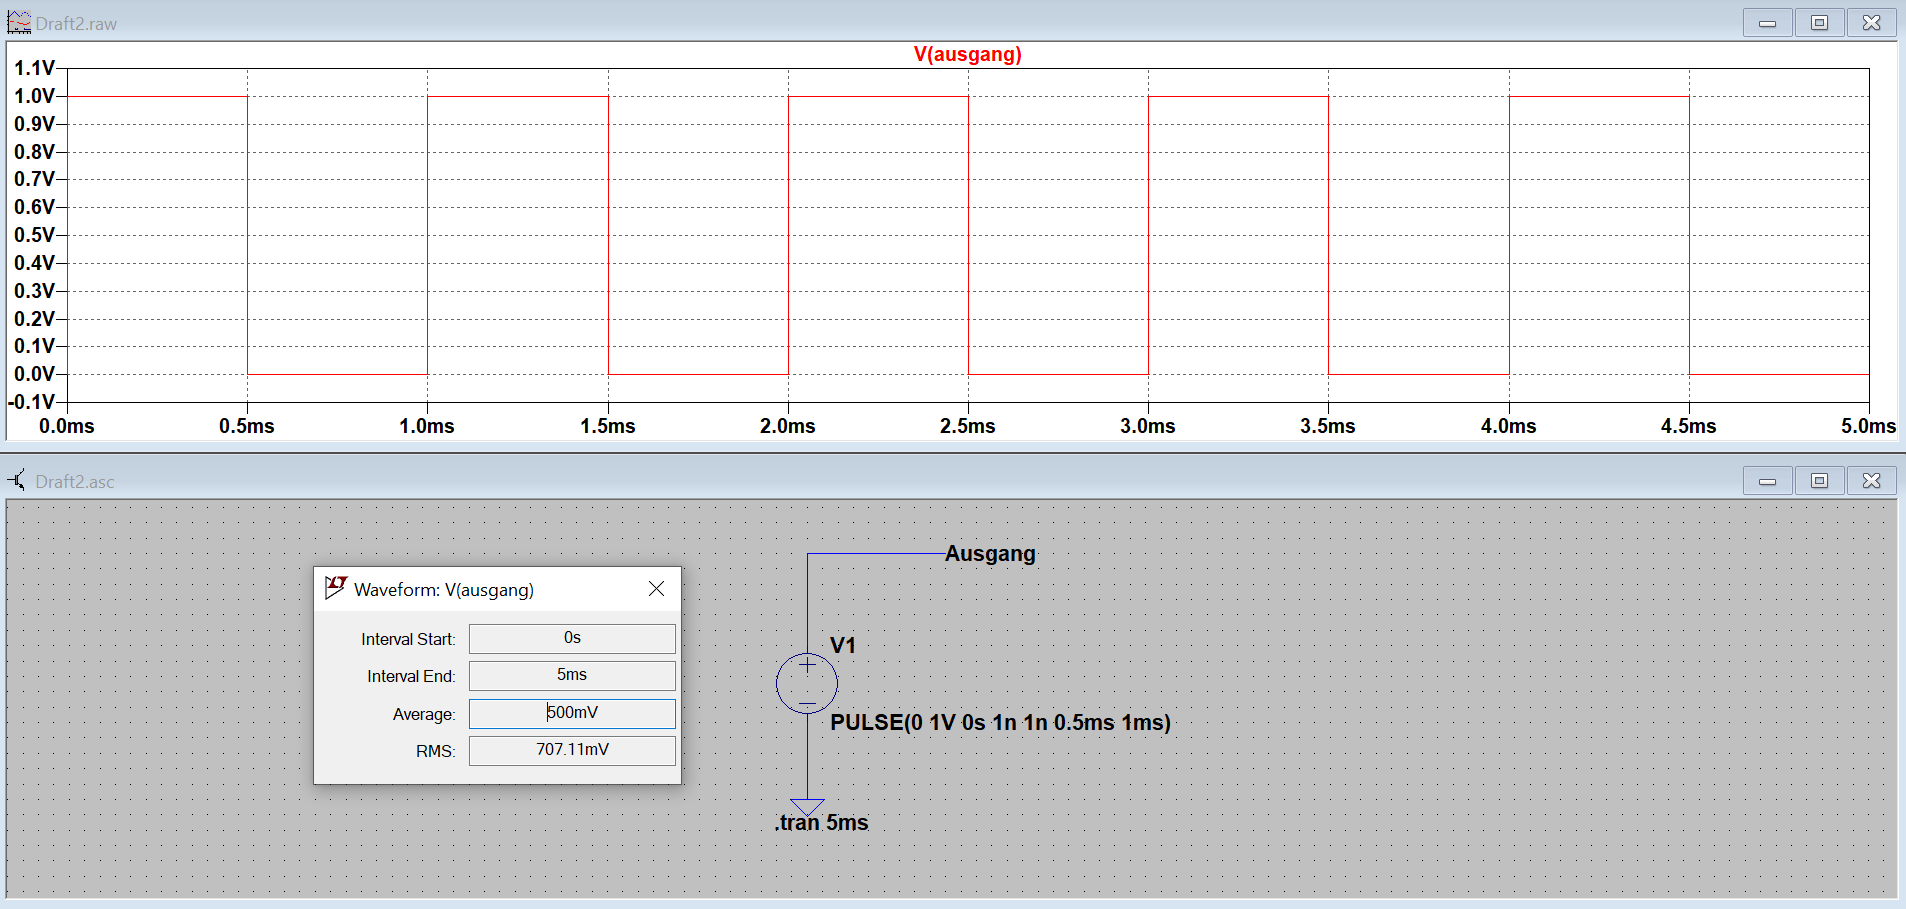
\includegraphics[scale=0.5]{213.PNG}
\caption{Symmetrisches Rechtecksignal mit $\^{U}=1V$, $T_{on}=0,5 ms$ und $f=1ms$}
\label{fig: symRechtecksignal}
\end{figure}

\subsection{Unsymmetrisches Rechtecksignal}
Zum Darstellen eines unsymmetrischen Recktecksignals wird ebenfalls der $T_{rise}$ und $T_{fall}$ Wert angepasst. Der liegt bei dieser Simulation bei jeweils 1ns. Durch eintragen der restlichen Werte \fref{fig: unsymRechtecksignal}, ergibt sich folgende LTSpice Simulation und Graph.
\begin{figure}[ht!]
\centering
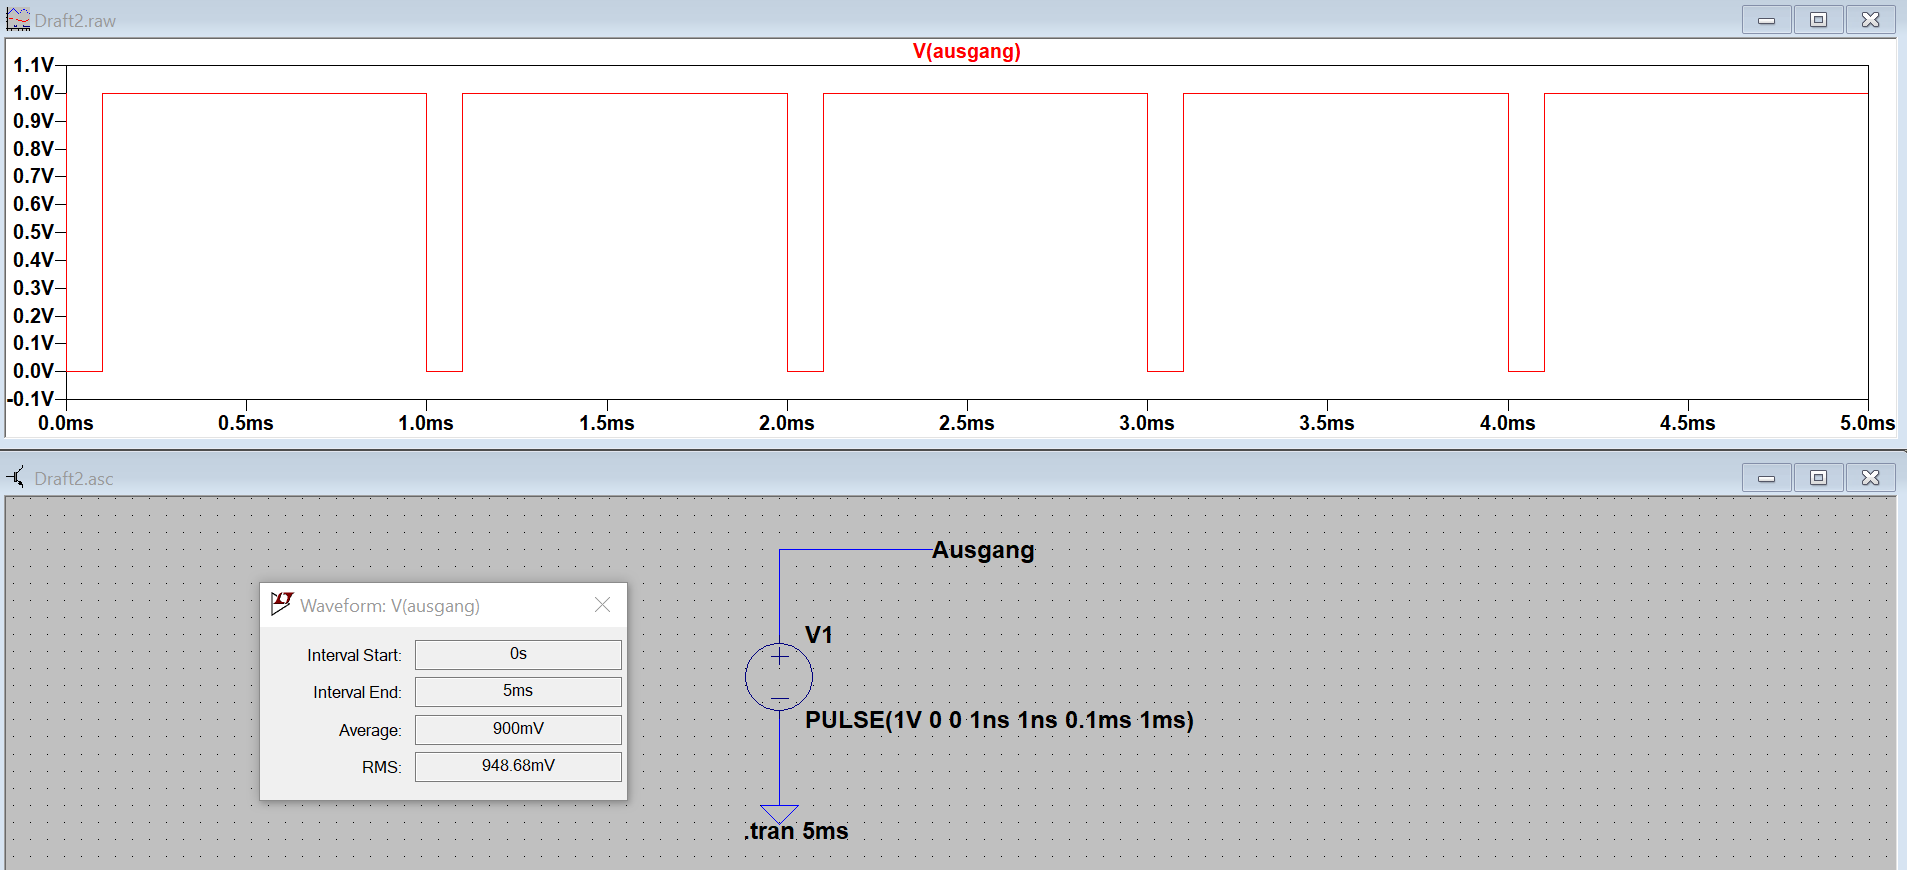
\includegraphics[scale=0.5]{214.PNG}
\caption{Unsymmetrisches Rechtecksignal mit $\^{U}=1V$, $T_{on}=0,1 ms$ und $f=1ms$}
\label{fig: unsymRechtecksignal}
\end{figure}

\subsection{Dreiecksignal}
Damit bei der Simulation mit LTSpice ein Dreiecksignal herauskommt, werden die Werte für $T_{rise}$, $T_{fall}$ und $T_{on}$ angepasst. 
$$T_{rise}=0.5ms$$
$$T_{fall}=0.5ms$$
$$T_{on}=0ms$$
Durch das einfügen der restlichen Werte \fref{fig: Dreiecksignal}, ergibt sich folgende LTSpice Simulation und Graph.
\begin{figure}[ht!]
\centering
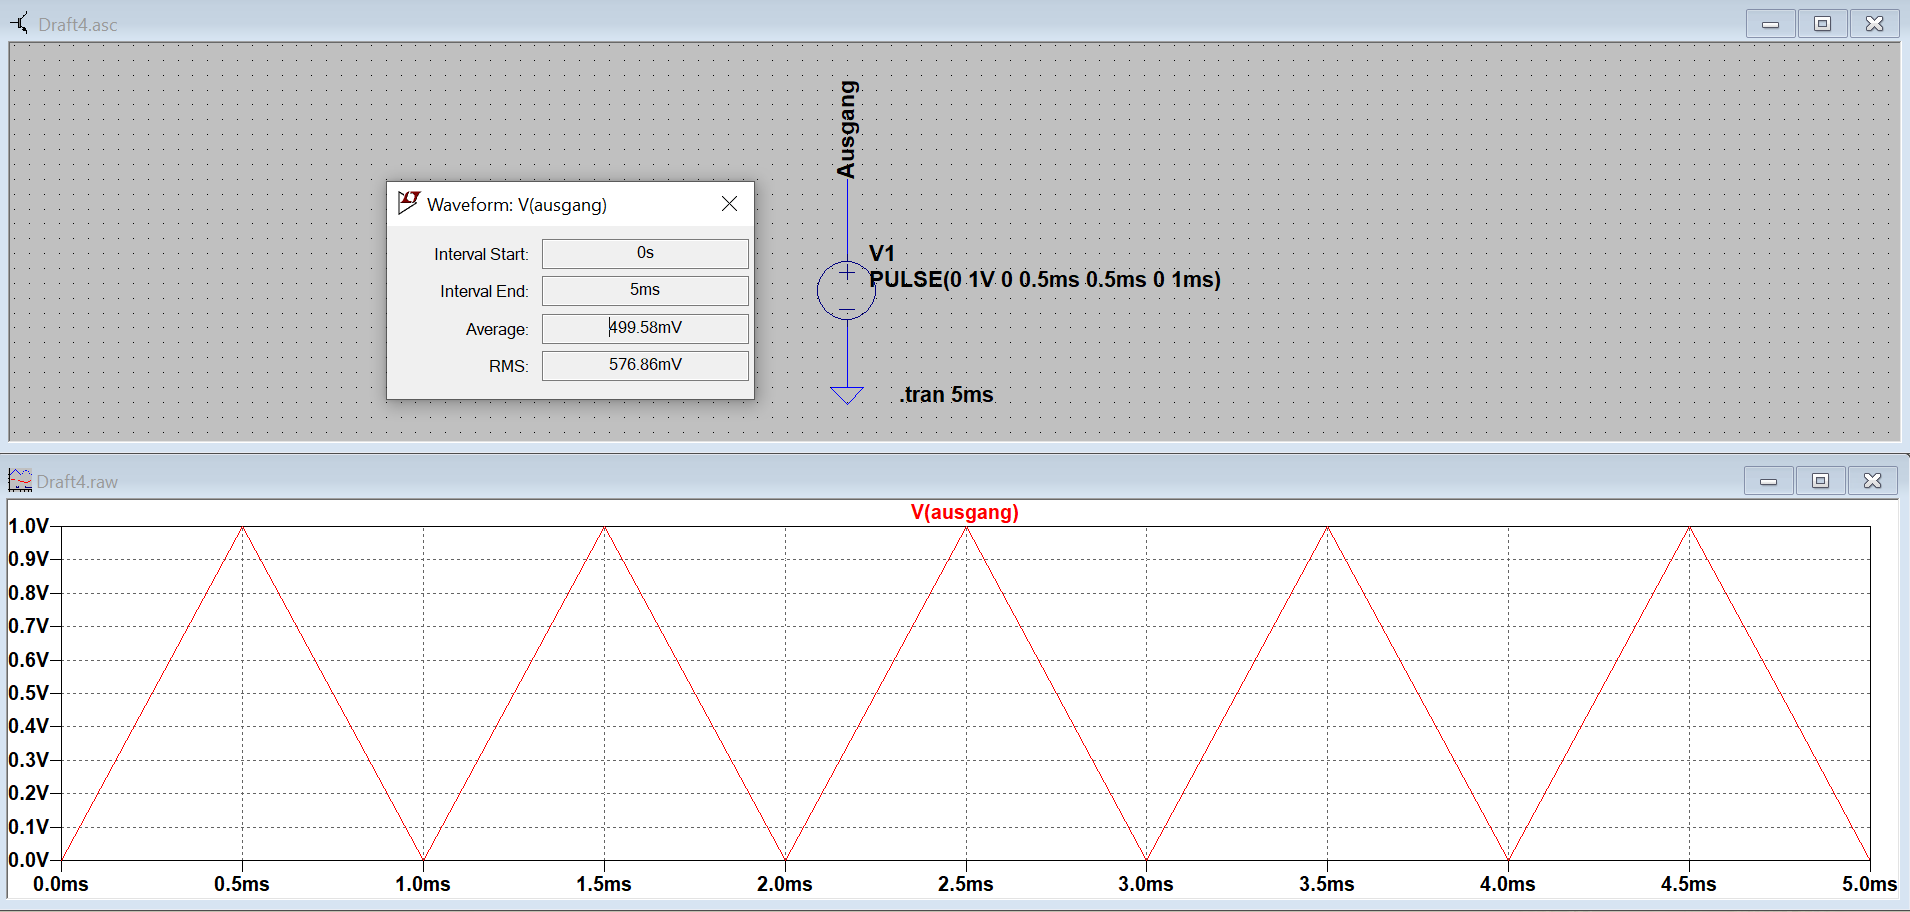
\includegraphics[scale=0.5]{215.PNG}
\caption{Dreiecksignal mit $\^{U}=1V$, $T=1ms$ }
\label{fig: Dreiecksignal}
\end{figure}
\newpage
\subsection{Sägezahnsignal}
Damit bei der Simulation mit LTSpice ein Dreiecksignal herauskommt, werden die Werte für $T_{rise}$, $T_{fall}$ und $T_{on}$ angepasst. 
$$T_{rise}=0.5ms$$
$$T_{fall}=1ns$$
$$T_{on}=0ms$$
Durch das einfügen der restlichen Werte \fref{fig: Sägezahnsignal}, ergibt sich folgende LTSpice Simulation und Graph.

\begin{figure}[ht!]
\centering
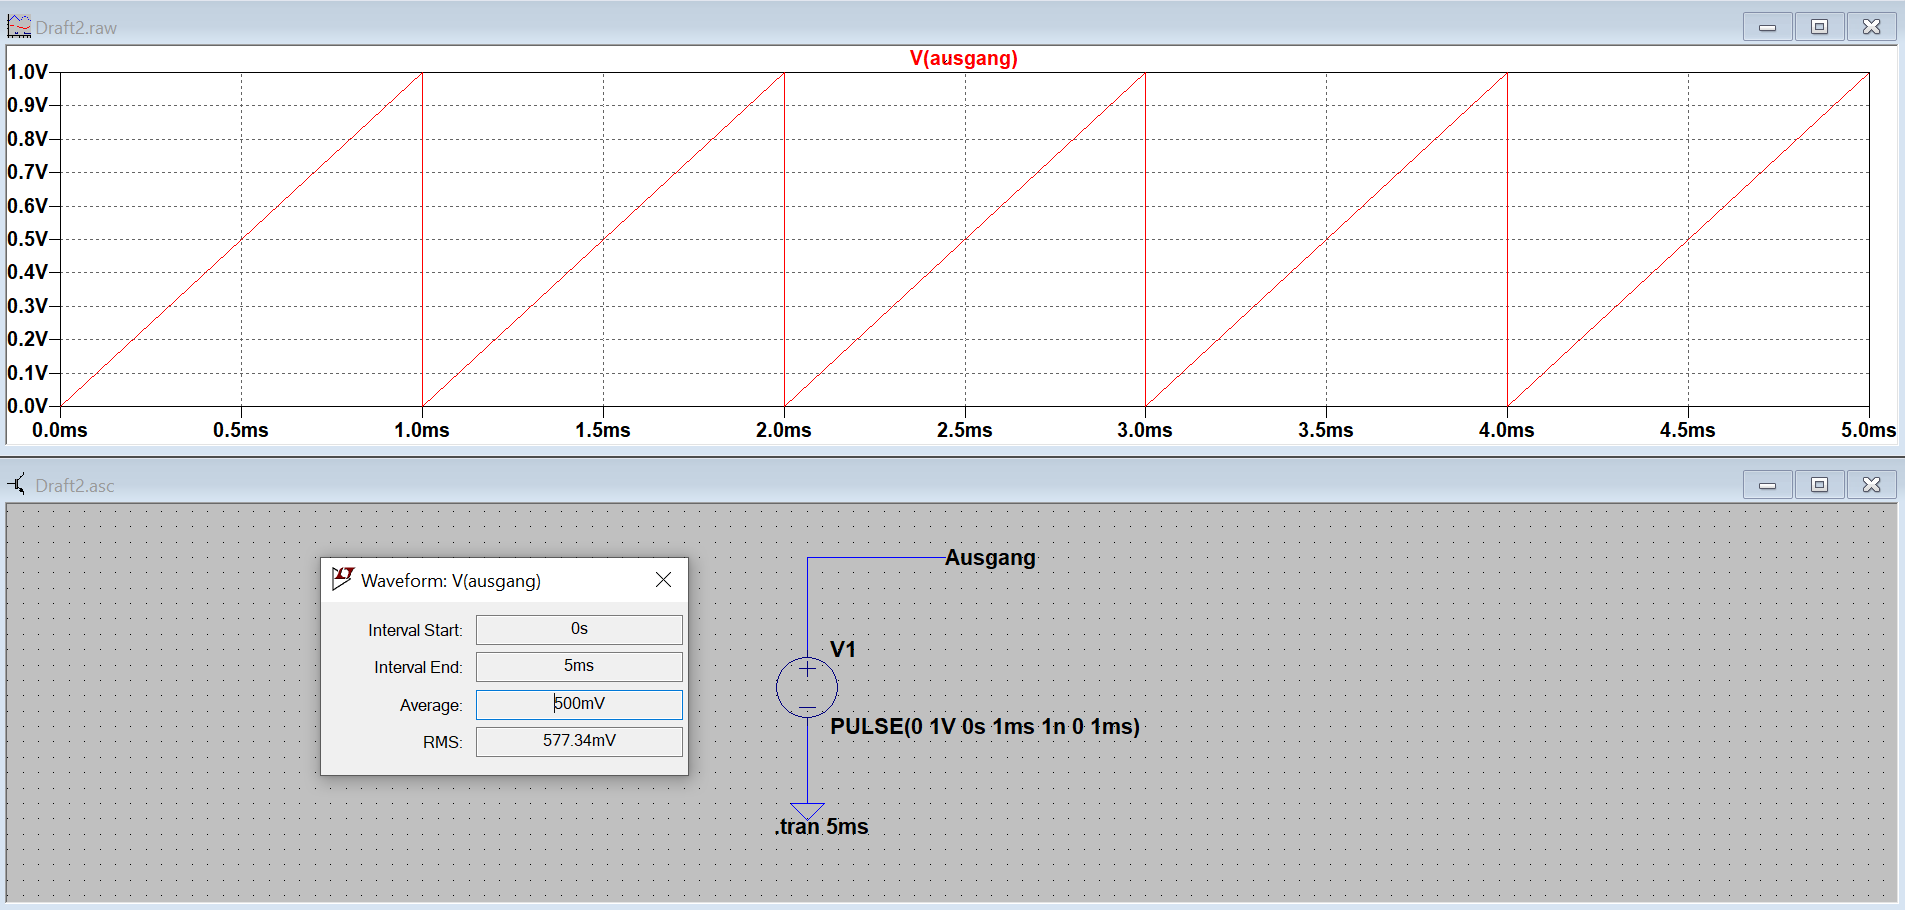
\includegraphics[scale=0.5]{216.PNG}
\caption{Sägezahnsignal mit $\^{U}=1V$, $T=1ms$}
\label{fig: Sägezahnsignal}
\end{figure}



Die von Hand ermittelten Effektivwerte (siehe Abschnitt 1.3) werden im Folgenden mit den Werten aus der Simulation verglichen. Die simulierten Effektivwerte sind auf den einzelnen Abbildungen \ref{fig: Signalquelle} bis \ref{fig: Sägezahnsignal} in den kleinen Kästchen unter RMS zu finden.
\begin{table}[ht!]
\centering
\caption{Wertetabelle für die Effektivwerte}
\label{fig: Effektivwerte}
\begin{tabular}{|c|c|c|} \hline
Signal & simulierte Effektivwerte & berechnete Effektiverte\\ \hline
Gleischspannungsquelle & 1V & 1V\\ \hline
Sinussignal & 707,19mV & 707mV\\ \hline
Symmetrisches Rechtecksignal & 707,11mV & 1V\\ \hline
Unsymmetrisches Rechtecksignal & 948,68mV & 1V\\ \hline
Dreiecksignal & 576,86mV & 578mV\\ \hline
Sägezahnsignal & 577,34mV & 578mV\\ \hline

\end{tabular}
\end{table}

Den Wert für das Sinussignal wurde in 1.3.1 Formel (1.9) berechnet. Der Wert für die Rechtecksignale sind in 1.3.2 Formel (1.17) und für die Dreiecksignale  in 1.3.3 Formel (1.26) zu finden. In Tab. \ref{fig: Effektivwerte} sind diese nochmal nebeneinander gestellt. Beim Vergleichen der Effektivwerte durch Berechnen und durch die Simulation ist direkt zu sehen, dass es dort kleine Unterschiede gibt. Bei dem Sinussignal und dem Dreiecksignal sind die Werte annäherungsweise gleich. Jedoch gibt es bei den Rechtecksignalen Unterschiede zwischen den Effektivwerten. Der des unsymmetrischen Dreiecksignals ist noch annäherungsweise an den errechneten 1V dran, der Effektivwert des symmetrischen Rechtecksignals hat jedoch einen Unterschied von fast 300mV. Dieser Wert passt eher zu dem berechneten Effektivwert des Sinussignals.

\newpage


\section{Spannungsteiler}
\subsection{Unbelasteter Spannungsteiler}
\begin{figure}[h!]
\centering
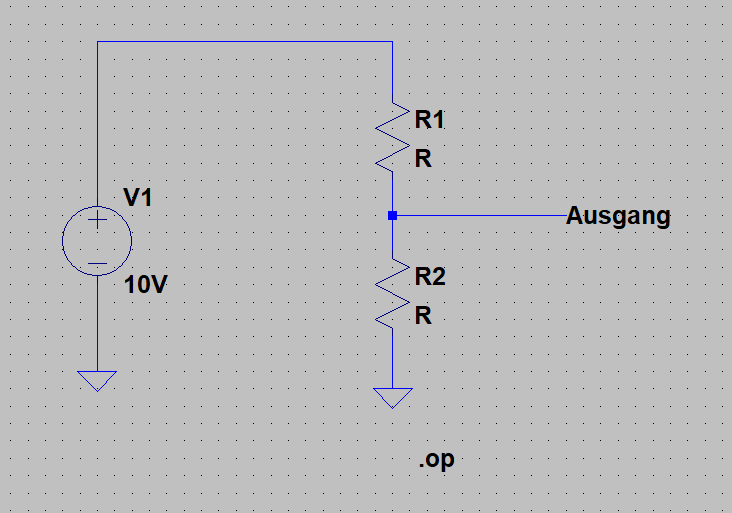
\includegraphics[scale=1]{221.PNG}
\caption{Unbelasteter Spannungsteiler}
\label{fig: Unbelasteter Spannungsteiler}
\end{figure}
Beim unbelasteten Spannungsteiler \fref{fig: Unbelasteter Spannungsteiler} werden jetzt die einzelnen Werte für $R_1$ und $R_2$ verändert und in die Schaltung eingegeben.

\begin{table}[h!]
\centering
\caption{Wertetabelle für den unbelasteten Spannungsteiler }
\label{fig: unbelasteter Spannungsteiler}
\begin{tabular}{|c|c|c|c|} \hline
$R_1$ in $\Omega$ & $R_2$ in $\Omega$ & $V_{aus}$ Simulation in V & $V_{aus}$ Spannungsteilerformel in V\\ \hline
$4,7k$ & $2,2k$ & 3,18841 & 3,18841\\ \hline
$47k$ & $22k$ & 3,18841 & 3,18841\\ \hline
$470k$ & $220k$ & 3,18841 & 3,18841\\ \hline
$4,7M$ & $2,2M$ & 3,18841 & 3,18841\\ \hline
$47M$ & $22M$ & 3,18841 & 3,18841\\ \hline

\end{tabular}
\end{table}

Mit der Spannungsteilerformel 
\begin{equation}
U_{aus}=U_{ges}\cdot \frac{R_2}{R_1+R_2}
\end{equation}
wird die Spannung am Ausgang von Hand berechnet. Dabei ist $U_{ges}=10V$, die Werte für $R_1$ und $R_2$ sind aus der Tabelle \ref{fig: unbelasteter Spannungsteiler} ablesbar.
Die Ergebnisse der Simulation und die Ergebnisse aus der Spannungsteilerformel sind identisch. Desweiteren sind die Ergebnisse für die verschiedenen Werte von $R_1$ und $R_2$ gleich, da diese Vielfache voneinander sind und sich somit die erhöhten Werte ausgleichen.

\subsection{Belasteter Spannungsteiler}
Der belastete Spannungsteiler ist wie der unbelastete Spannungsteiler aufgebaut, jedoch wird an den Ausgang ein Innenwiderstand von $R_3=10M\Omega$ dazugeschaltet. Dies ist in Abb.\ref{fig: bel.Spannungsteiler} veranschaulicht.
\begin{figure}[h!]
\centering
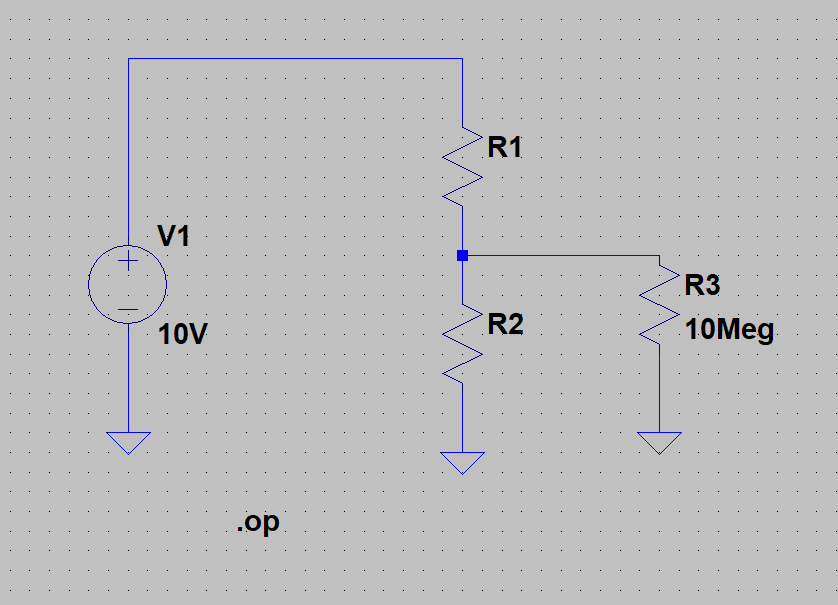
\includegraphics[scale=1]{222.PNG}
\caption{Belasteter Spannungsteiler}
\label{fig: bel.Spannungsteiler}
\end{figure}

\begin{table}[h!]
\centering
\caption{Wertetabelle für den unbelasteten Spannungsteiler }
\label{fig: belasteter Spannungsteiler}
\begin{tabular}{|c|c|c|} \hline
$R_1$ in $\Omega$ & $R_2$ in $\Omega$ & $V_{aus}$ Simulation in V \\ \hline
$4,7k$ & $2,2k$ & 3.18793\\ \hline
$47k$ & $22k$ & 3.18363\\ \hline
$470k$ & $220k$ & 3.14133\\ \hline
$4,7M$ & $2,2M$ & 2.77288\\ \hline
$47M$ & $22M$ & 1.2761\\ \hline

\end{tabular}
\end{table}

Beim Vergleichen der Ausgangsspannung $V_{aus}$ der Simulation (siehe Tab.~\ref{fig: belasteter Spannungsteiler} und~\ref{fig: unbelasteter Spannungsteiler})fällt auf das die Werte voneinander abweichen. Das liegt daran, das ein nicht variabler Widerstand $R_3=10M\Omega$ (Innenwiderstand des Voltmeters) parallel zu $R_2$ dazugeschaltet ist. Da dieser immer den gleichen Wert besitzt, jedoch die Werte für $R_1$ und $R_2$ steigen, verändert sich auch die Spannung am Ausgang. Dies  ist auch an der Formel für einen belasteten Spannungsteiler zu sehen.
\begin{equation}
U_{aus}=U_{ges}\cdot \frac{R_2||R_3}{R_1+(R_2||R_3)}
\end{equation}
Hier wird der Widerstand $R_3$ parallel zu $R_2$ geschaltet und  mit dem festen Wert für $R_3$ gerechnet. Dadurch sinkt die Spannung bei höheren Widerstandswerten von $R_1$ und $R_2$.

\section{Potentiometer}
\begin{figure}[h!]
\centering
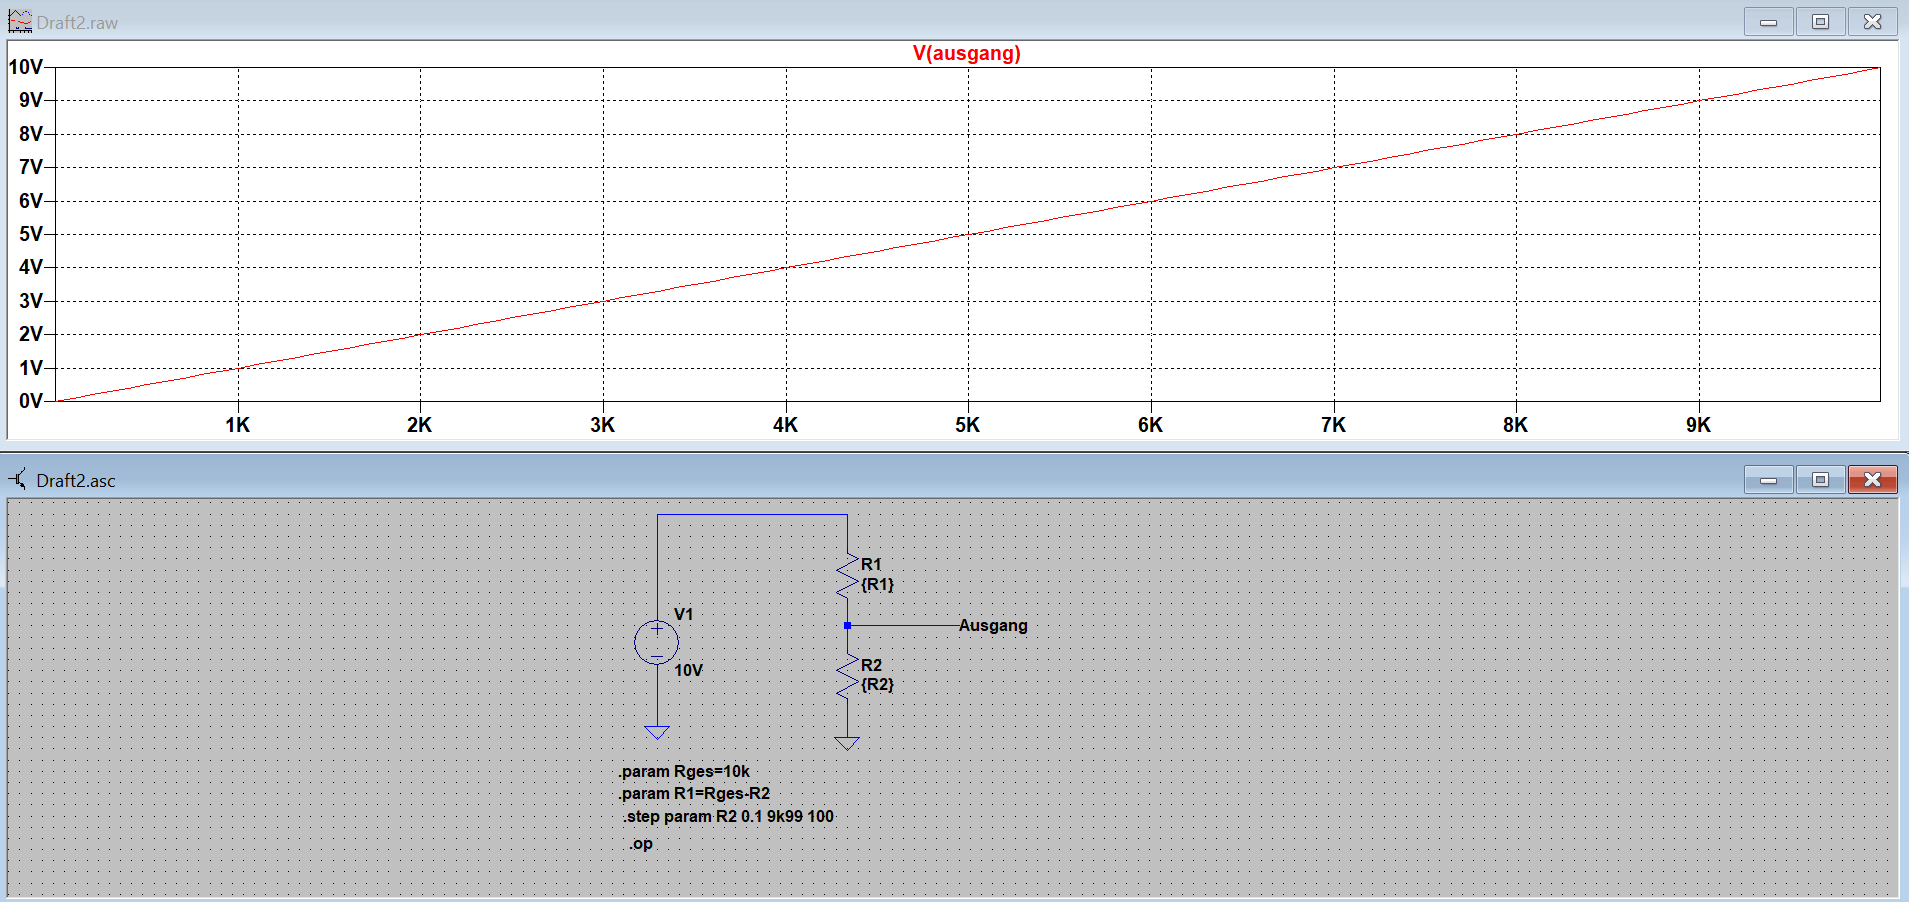
\includegraphics[scale=0.5]{23.PNG}
\caption{Darstellung eines Potentiometers}
\label{fig: Potentiometer}
\end{figure}

Die Schaltung in Abb.~\ref{fig: Potentiometer} sieht aus wie die Abb.~\ref{fig: Unbelasteter Spannungsteiler} eines unbelasteten Spannungsteilers. Jedoch ist beim Potentiometer der Widerstand $R_1$ vom Widerstand $R_2$ abhängig.
\begin{equation}
R_1=R_{ges}-R_2
\end{equation}
Die Werte von $R_2$ ändern sich dabei in $100\Omega$ Schritten im Intervall von $0.1\Omega$ bis $9k99\Omega$, unter der Bedingung:
$$0\Omega \leq R_2\leq R_{ges}$$
Die Simulation beginnt mit $0.1\Omega$ und endet mit $9k99\Omega$ damit $R_1$ nicht $0\Omega$ wird.\\
Im Graphen \fref{fig: Potentiometer} ist zu sehen, das mit steigendem $R_2$ auch die Ausgangsspannung $V_{aus}$ steigt.








        \chapter{Fazit}
Bei dem Versuch werden erstmal die Grundlegenden Begriffe der Gleich- und Wechselspannung erklärt. 
Diese sind dann durch ein Voltmeter in die Schaltungen eingebracht worden. 
Dabei sind Schaltungen wie der Spannungsteiler und das Potentiometer aufgebaut worden 
und durch LTSpice simuliert. Zum besseren Verständnis des Graphen wurde 
dann der Effektivwert sowie die Ausgangsspannung per Hand ausgerechnet und mit den von 
LTSpice simulierten Werten verglichen. Die Werte für den Spannungsteiler und den Potentiometer
 haben mit den zu erwarteten Werten wunderbar funktioniert. Bei dem Rechtecksignal einer 
 Spannungsquelle sind jedoch zwischen simuliertem und berechneten Effektivwert Differenzen 
 aufgetreten. Ursprung des Fehlers kann in der Rechnung liegen, obwohl diese öfters zum Überprüfen 
 der Richtigkeit durchgeführt wurde. Der Fehler kann auch in der falschen Durchführung von 
 LTSpice liegen. In der Aufgabenstellung von 2.1 (Signalquellen), war nicht genau ersichtlich ob 
 das Voltmeter durch eine Wechselspannung oder Gleichspannung angetrieben wird. Durch eine 
 Wechselspannung würde der Graph von -1V bis 1V gehen. Die simulierten Graphen in dem Bericht 
 sind jedoch nur von 0V bis 1V aufgetragen. Durch die Wechselspannung sind die berechneten Werte 
 aber auch nicht zu erzielen, da diese ebenfalls zur Lösung des Problems simuliert wurden und 
 nicht mit den berechneten Werten übereinstimmen. 
    
    
    
    %\printbibliography
\end{document}